% !TEX root = report.tex

\chapter{Bot Architecture}

This chapter will describe the overall structure of \massexpand and provide descriptions of the major components.

\section{Overall Structure}

The starting point of the creation of the bot was the example AI module distributed with BWAPI. The example contains the main update loop of the bot, all event listeners BWAPI supports and methods for drawing extra information on the screen. It also provides some sample code for giving orders to units. We left the example module mostly intact, except for the units orders which we removed completely. We added calls to methods of a new class, HighCommand, which would be the control center for our code. The main benefits of this were that we kept the example code for reference, and that if there would be a major change in BWAPI, we could use the new example module and quickly plug in our own code.

In our first attempts to create a bot, we tried using BWSAL, a collection of classes forming an abstraction layer for BWAPI. These classes provide methods for common tasks such as assigning workers to collect resources, maintaining a build queue and finding suitable building places. We quickly abandoned BWSAL after realizing it would be hard to adapt it to our ideas. What we kept from BWSAL were two helper classes, UnitGroup (an excellent class to select and divide groups of units) and BuildingPlacer (a class with methods to determine where a building should be built). We also kept the overall structure BWSAL used, including the naming scheme (the "managers").

The managers are all responsible for a part of the performance of the bot. For example, we have a manager keeping track of our minerals and gas, a manager storing information about enemy units and a manager overseeing construction of buildings and units. Organizing the bot this way allows us to seperate code pertaining to different areas of the bot operation, and also allows us to structure the way the information obtained from the game flows through our bot, resulting in commands sent back to the game. This flow of information is shown in Figure~\ref{fig:flowofinformation}.

\begin{figure}[htb]
\centering
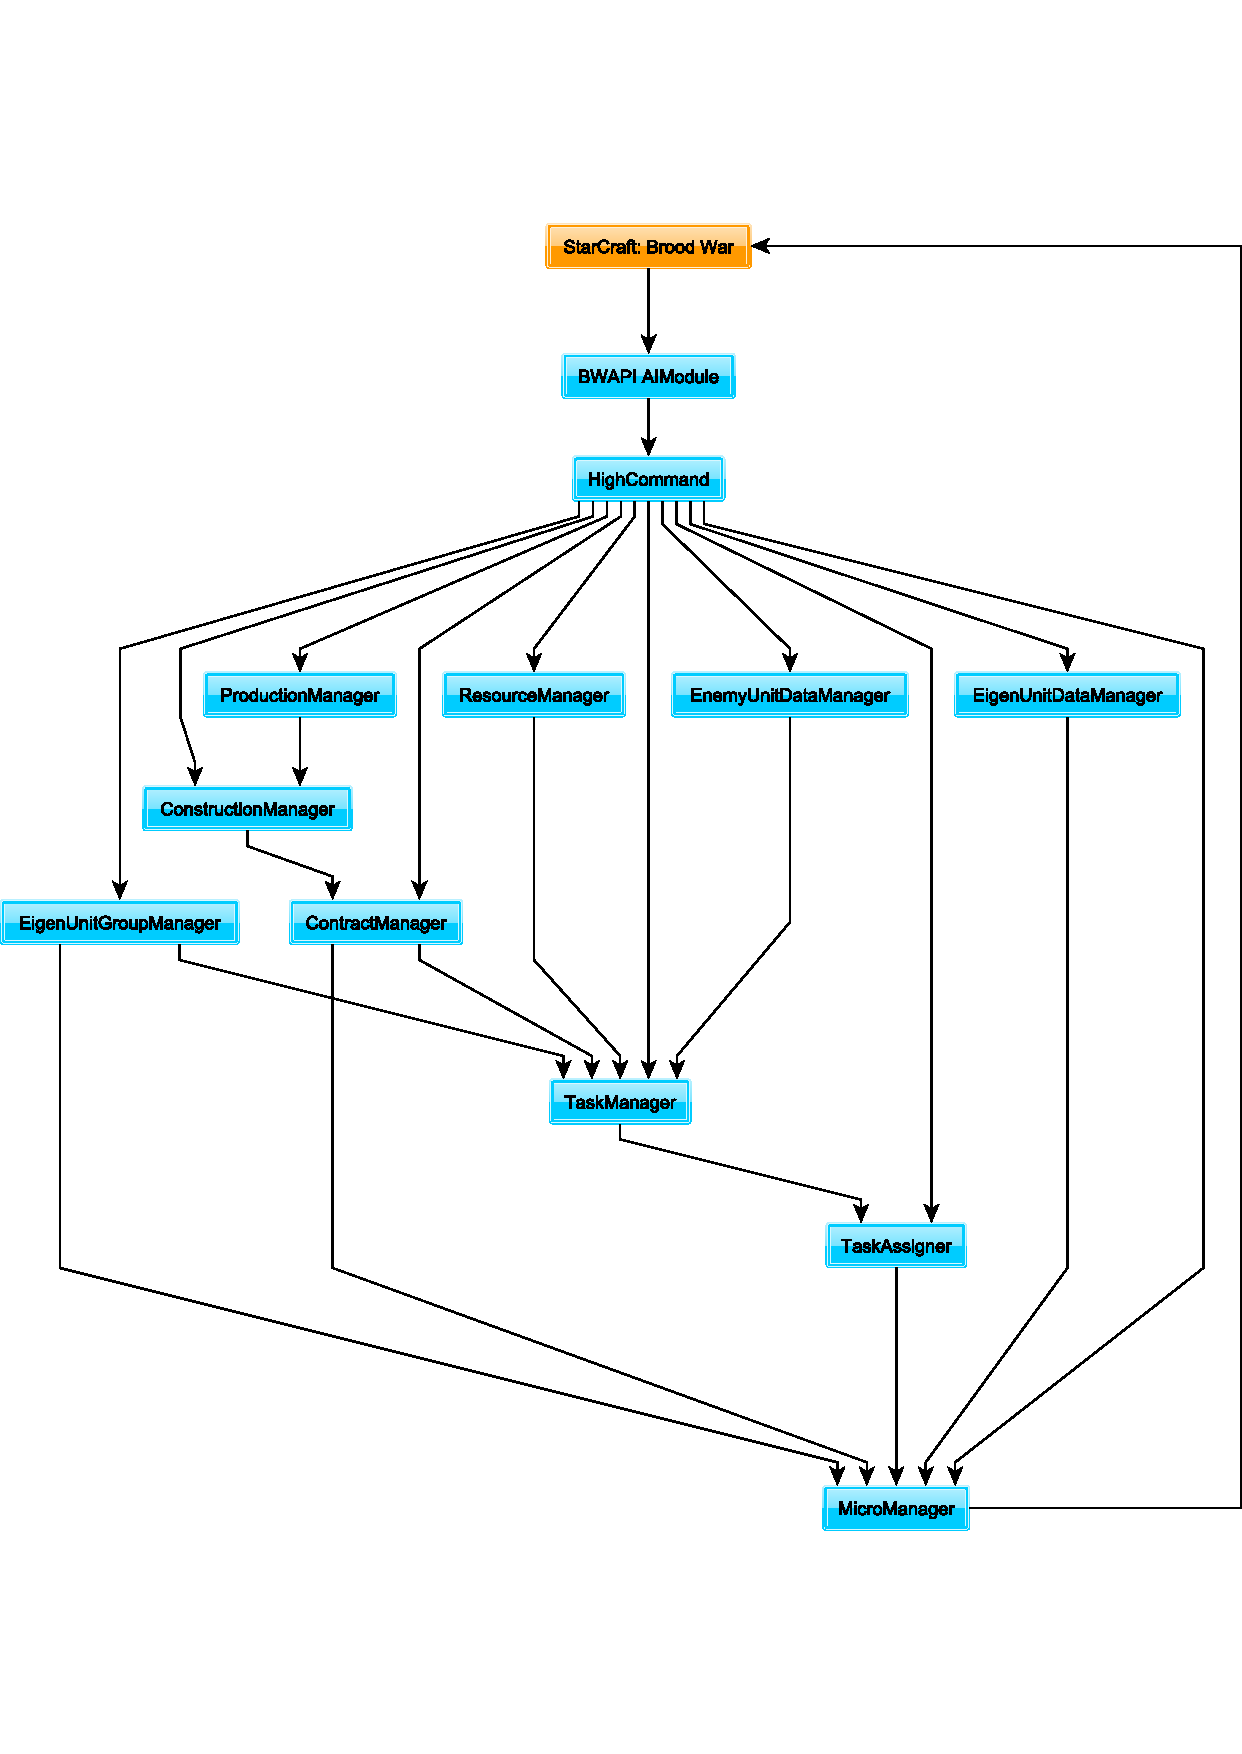
\includegraphics[width=\textwidth, trim= 0mm 30mm 0mm 30mm, clip]{images/flowofinformation}
\caption{The flow of information from StarCraft through Mass Expand to MicroManager and ConstructionManager, which send commands back to StarCraft.}
\label{fig:flowofinformation}
\end{figure}

Figure~\ref{fig:flowofinformation} can also be seen as a parallelized version of the main loop of our bot. However, in practice, the managers are called in serial form. When the update function of HighCommand is called (which is our main loop), it tells the managers to update in the following order:

\begin{description}
\item[EigenUnitDataManager] Data about our own units is updated.
\item[EigenUnitGroupManager] Any new units we have are assigned to persisting unitgroups, small groups are merged and large groups are split up.
\item[ResourceManager] Lists of mineable gas and mineral deposits close to our bases are updated.
\item[EnemyUnitDataManager] Data about visible enemy units is updated, such as their position and health.
\item[ProductionManager] Plans are made for the construction of buildings, units, upgrades and technology.
\item[ConstructionManager] Plans made by ProductionManager are executed if possible.
\item[ContractManager] Build orders for buildings are delegated to drones and a suitable build location is found for them.
\item[TaskManager] Tasks are collected from the other managers.
\item[TaskAssigner] The collected tasks are assigned to units and unitgroups.
\item[MicroManager] Mobile units are given specific movement instructions, based on their tasks and enemies near their location.
\end{description}

HighCommand and the managers will be described in more detail in the following sections.

\section{HighCommand}

HighCommand is the control center of our bot. It does three things:

\begin{itemize}
\item It instantiates the managers and calls them in the right order.
\item It listens for game events from BWAPI and forwards them to the right managers.
\item It draws extra textual and graphical information on top of the game interface.
\end{itemize}

The specific order in which HighCommand calls the managers is listed in the previous section. The order is important because some managers require updated information from other managers to function.

BWAPI allows AI modules to draw extra information on the screen, on top of the game interface. This is a handy feature to show internal information of the bot that would otherwise be invisble. HighCommand currently calls these functions to display the location and type of tasks, the assignment of units to tasks (shown as lines from units to tasks), the build queue and current contracts (drones that are ordered to build a structure).

\section{EigenUnitDataManager}

EigenUnitDataManager records data about our own units (\emph{eigen} means own in Dutch). BWAPI provides many methods to get data about our own units, but this data might change each frame. By recording data from the last frame, we are able to detect changes. One of such changes we monitored was a loss of hit points, which indicated a unit was being attacked (BWAPI later added a function to detect whether a unit was under attack). Another option this manager provides is to record which of our units were seen by the enemy and where and when this occured. If one of our units ever moved within visual range of an enemy unit, we can be sure the enemy knows about that unit and will act on that information. On the other side, we can use unseen units to our advantage (such as using them for a surprise attack).

\section{EigenUnitGroupManager}

This manager divides all our mobile units into persistent groups. Such groups can be manipulated as if it were a single unit: orders given to a unitgroup are passed to all the units in the group. Unitgroups are implemented in the UnitGroup class from BWSAL, which provides many helpful selector functions, such as "get all flying units in this group". The selector functions can be chained, allowing us to manage our units with very concise code.

The groups that the EigenUnitGroupManager maintains are updated whenever the number of units we have is changed. When a new unit is created, it is either assigned to an existing group or given its own new group. When one of our units dies or we otherwise lose control of it, it is removed from its group. The groups are then balanced by reassigning units between groups, according to various rules.

For example, new Overlords are always given a new group of their own. However, if there is a group of Mutalisks that does not have any Overlords, the Overlord will be moved to the Mutalisk group in the balancing step. It is handy to have a Overlord with Mutalisks (both flying units) because the Overlord can detect stealth units, which are then easily taken out by the Mutalisks.

Drones are a special case. We keep all Drones in a single group. While they are capable of combat, they are mostly used for gathering resources and construction. By keeping them in a special group we make sure they are not accidentally assigned to combat tasks. The drone group has a constant pointer, allowing easy access to all drones.

\section{EnemyUnitDataManager}

EnemyUnitDataManager keeps track of enemy units. By default, BWAPI only allows access to visible units. However, we we want to retain information about them when they become inaccessible, such as when they use a stealth ability or move into fog of war. Units can also transform into a different unittype. In that case, we need to make sure we recognize it as the same unit instead of counting it as two seperate units. The manager currently records five pieces of information about each enemy unit we encounter: its type, its hitpoints, its position, its last known position, and the time at which it was last seen by us. This information is saved together with a pointer to the unit.

There is an important difference between the position and the last known position. While an enemy unit is visible, we update its position, and its last known position is changed to that position. When it moves somewhere we cannot see it (for example, into fog of war) we change its position to "unknown" and keep its last known position. We can then send scouts to make that position visible. If the unit is still there, we can update its position again.

\section{ResourceManager}

\section{TaskManager}

\section{TaskAssigner}

\section{ProductionManager}

\section{ConstructionManager}

\section{ContractManager}

\section{MicroManager}